\documentclass[compress,10pt]{beamer}
% version imprimable pour assistance
%\documentclass[10pt, green, handout]{beamer}
\usepackage[T1]{fontenc}
\usepackage[utf8]{inputenc}
\usepackage[frenchb]{babel} % le document est en français
\usepackage{rotating,amsmath}
\usepackage{graphicx,cancel}       % pour ins\'erer des figures


        % pour d\'efinir plus de couleurs
\usetheme[subsectionpage=progressbar]{metropolis}
\setbeamertemplate{section in toc}[sections numbered]
\setbeamertemplate{subsection in toc}[subsections numbered]

%\usetheme{metropolis}  %Applique le theme INRA (ce dernier doit être present dans le repertoire courant)
\usepackage{xcolor,colortbl}
\usepackage{array}
\usepackage{mdframed}
\usepackage{multirow}
\usepackage{lmodern}	
\usepackage{tikz}
\usetikzlibrary{positioning,shapes,arrows}



\setbeamerfont{bibliography item}{size=\tiny}
\setbeamerfont{bibliography entry author}{size=\tiny}
\setbeamerfont{bibliography entry title}{size=\tiny}
\setbeamerfont{bibliography entry location}{size=\tiny}
\setbeamerfont{bibliography entry note}{size=\tiny}
            

\definecolor{dgreen2}{RGB}{102,193,191}
%RGB()
\definecolor{dgreen}{RGB}{255,165,0}
\definecolor{mygrey}{RGB}{230,230,230}


\setbeamertemplate{blocks}[rounded][shadow=true]
\setbeamercolor{block title}{use = structure  ,bg=mygrey, fg=dgreen}
%\setbeamercolor{normal text}{fg=black,bg=white}
%\setbeamercolor{alerted text}{fg=lgreen}
%\setbeamercolor{example text}{fg=lgreen}
%\setbeamercolor{structure}{fg=dgreen} %d'où ce bleu par défaut
\setbeamercolor{background canvas}{parent=normal text}


\usepackage{tikz}
\usetikzlibrary{calc,shapes,backgrounds,arrows,automata,shadows,positioning}
\setbeamertemplate{frametitlecontinuation}{\insertcontinuationcountroman}

%-------------------------------------------------------------------------------
% Quelques options pdf
%-------------------------------------------------------------------------------
\hypersetup{
pdfpagemode = FullScreen, % afficher le pdf en plein \'ecran
pdfauthor   = {},%
pdftitle    = {},%
pdfsubject  = {},%
pdfkeywords = {Science,Impact},%
pdfcreator  = {PDFLaTeX,emacs,AucTeX},%
pdfproducer = {INRAE}%
}


\newcommand\Wider[2][3em]{%
\makebox[\linewidth][c]{%
  \begin{minipage}{\dimexpr\textwidth+#1\relax}
  \raggedright#2
  \end{minipage}%
  }%
}

%\AtBeginSection[]
%{  \begin{frame}
%  \frametitle{}
%  \tableofcontents[currentsection, hideothersubsections]
%  \end{frame} 
%}

% \AtBeginSubsection[]
% {  \begin{frame}
%   \frametitle{}
%   \tableofcontents[currentsection, hideothersubsections]
%   \end{frame} 
% }


%
\usepackage{amsmath}
\DeclareMathOperator*{\argmax}{arg\,max}
\DeclareMathOperator*{\argmin}{arg\,min}
\newcommand{\bX}{\boldsymbol{Y}}
\newcommand{\pr}{\mathbb{P}}
\newcommand{\E}{\mathbb{E}}

\newcommand{\Xall}{\bX}

\newcommand{\Zall}{\bZ}
\newcommand{\M}{\mathcal{M}_{Q}}
\newcommand{\ind}{\mathds{1}}
\newcommand{\Mcal}{\mathcal{M}}
\newcommand{\Qcal}{\mathcal{Q}}
\newcommand{\colSBM}{colSBM}

\newcommand{\bZ}{\boldsymbol{Z}}
\newcommand{\bpi}{\boldsymbol{\pi}}
\newcommand{\balpha}{\boldsymbol{\alpha}}
\newcommand{\btau}{\boldsymbol{\tau}}


\def\Ecal{\mathcal{E}}



\def\N{\mathbb{N}}
\def\R{\mathbb{R}}
\def\F{\mathcal{F}}
\def\Nb{\boldsymbol{N}}
\def\bZ{\boldsymbol{Z}}
\def\btheta{\boldsymbol{\theta}}
\def\bpi{\boldsymbol{\pi}}
\def\bY{\boldsymbol{Y}}
\def \ind{\mathbb{I}}
\def \P{\mathbb{P}}
\def \pen{\mbox{Pen}}
\def \SBM{\mbox{SBM}}

\newcommand{\lat}{\mathbf{Z}}
\newcommand{\Xm}{Y^{m}}
\newcommand{\Zm}{Z^{m}}
\newcommand{\pim}{\pi^{m}}
\newcommand{\alpham}{\alpha^{m}}
\newcommand{\taum}{\tau^{m}}
\newcommand{\con}{\alpha}
\newcommand{\conm}{\alpha^{m}}
\newcommand{\dens}{\delta}
\newcommand{\nm}{n_m}



%------------------------------------------
% \title{Some works on the modeling of multi-layer networks by stochastic block models}
% \subtitle{Application in ecology and sociology}
% % \date{\today}
% \date{Séminaire Parisien de Statistique. IHP. Octobre 2021}
% \author{Sophie Donnet. MIA PARIS(-SACLAY), INRAE. }
% \institute{}
% \titlegraphic{\hfill
\includegraphics[height=0.4cm]{Logo-INRAE}}


\title{A gentle introduction to the Variational Neural Networks}
\author{J. Aubert and S. Donnet for StateOfTheR}
\date{Dec.~2021}

\begin{document}
\frame{\titlepage}



%#######################################
\begin{frame}{Context}

\begin{itemize}
\item  In statistical learning, two main tasks:
\begin{itemize}
 
\item   \textbf{Regression or classification}
\item   \textbf{Reduction of dimension}
 
\end{itemize}
  Neural networks are used to construct the regression function,
  classifier or encoder-decoder (\textbf{autoencoder}).
\item
  \textbf{Variational versions} are used when we do not want to optimize
  a parameter but a \textbf{probability distribution}
\begin{itemize}
  \item
  if one wants to structure the latent space
\item
  if one wants to perform Bayesien inference
  \end{itemize}
  
\item
  Relies on
  \begin{itemize}
\item
  \textbf{Neural networks} : we know already
\item
  \textbf{Variational EM algorithm}: we know already, but anyway it is
  not complicated
   \end{itemize}
\end{itemize}
\end{frame}


%###############################################
\begin{frame}
\frametitle{Overview} 
\tableofcontents
\end{frame}


%#######################################

\section{Basics on regression, classification, reduction of dimension}

\begin{frame}{Regression or classification}
\begin{itemize}

\item
  Let \((\mathbf{X},\mathbf{Y})\) be our dataset:

  \begin{itemize}
  \item
  \((\mathbf{X},\mathbf{Y})=(X_i, Y_i)_{i \in 1, \dots,N_{obs}}\)
\item
  \(\forall i =1,\dots,N_{obs}\), \textbf{Variables}
  \(X_i \in \mathbb{R}^n\).\\
\item
  \(Y_i \in \mathcal{Y}\) the variable to explain :
  \textbf{classification} or \textbf{regression}
\end{itemize}
\item  Looking for a function \(f\)  \textbf{classifier} or \textbf{regression}

\begin{itemize}
 \item
 
  \(f :\mathbb{R}^n \mapsto \mathcal{Y}\) and
\item
  such that
  \[Y \approx f(X) \Leftrightarrow \mbox{Loss}(Y -   f(X)) \mbox{ small } \]
\item
  If \textbf{regression} \(\mbox{Loss}(Y - f(X)) = ||Y - f(X)) ||^2\)
\item
  If \textbf{classification} : Loss = cross-entropy
\end{itemize}
\end{itemize}
\end{frame}
%#######################################

\begin{frame}{Regression or classification}
\begin{figure}

{\centering 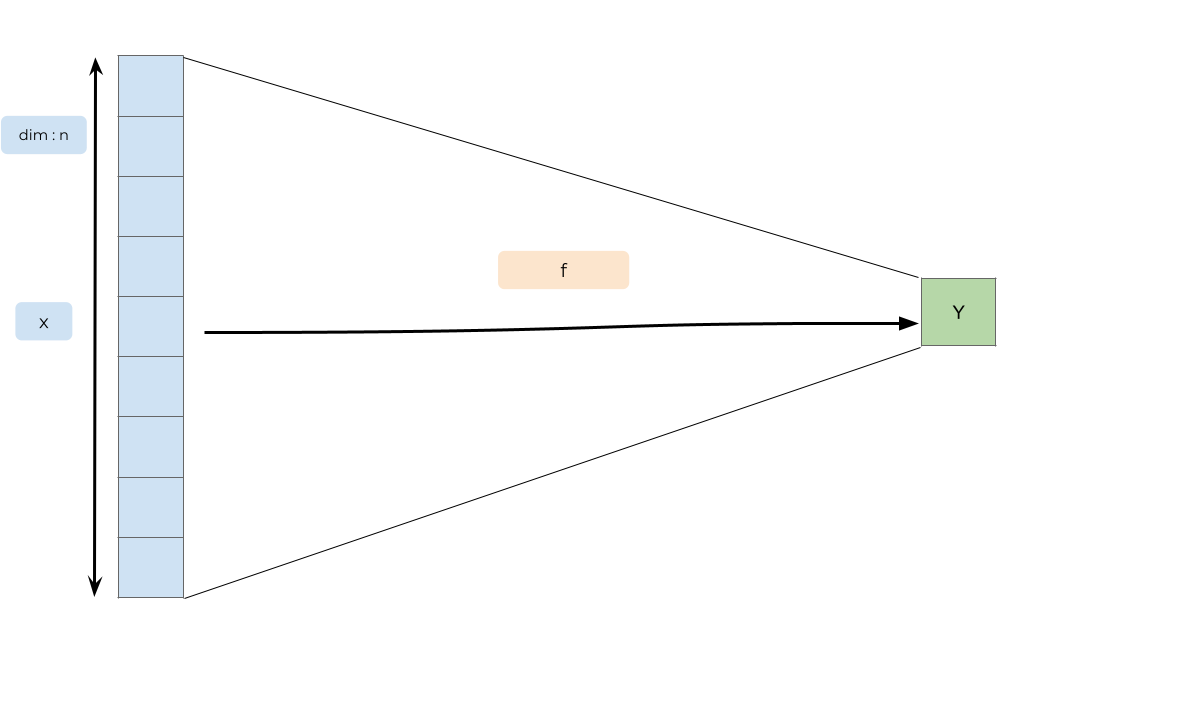
\includegraphics[width=0.9\linewidth]{images/RegressionClassification} 

}


\end{figure}
\end{frame}

\begin{frame}{Reduction of dimension}

\textbf{Autoencoders} are used for the reduction of dimension of
(large) datasets.

Let \(X\) be our dataset:
\(\mathbf{X}=(X_i)_{i \in 1, \dots,N_{obs}}\)

\begin{itemize}
\item
  \(\forall i =1,\dots,N_{obs}\), \(X_i \in \mathbb{R}^n\).
\item
  Looking for two functions
  \begin{itemize}
\item
  \textbf{Encoder} \(e :\mathbb{R}^n \mapsto \mathbb{R}^m\) and
\item
  \textbf{Decoder} \(d :\mathbb{R}^m \mapsto \mathbb{R}^n\)
\end{itemize}
  \item
  such that
  \[X \approx d(e(X)) \Leftrightarrow ||X -   d(e(X)) ||^2 \mbox{ small } \]
\item
  \(Z = e(X)\) : \textbf{latent variable}
\end{itemize}
\end{frame}

%#######################################




\begin{frame}{Autoencoder}
\begin{figure}

{\centering 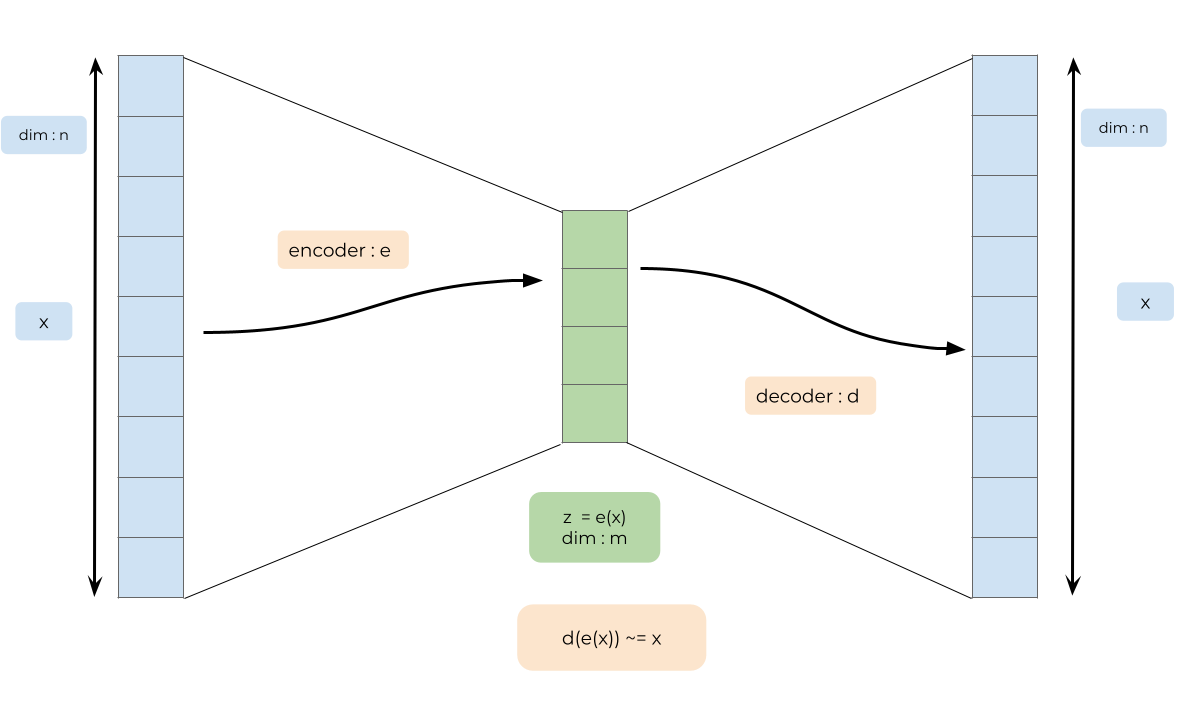
\includegraphics[width=0.9\linewidth]{images/Autoencoder} 

}
\end{figure}
\end{frame}
%#######################################

\section{Neural networks}

\subsection{Definition of neural networks}
\begin{frame}{About \(f\): neural networks}
\protect\hypertarget{about-f-neural-networks}{}
\begin{figure}

{\centering 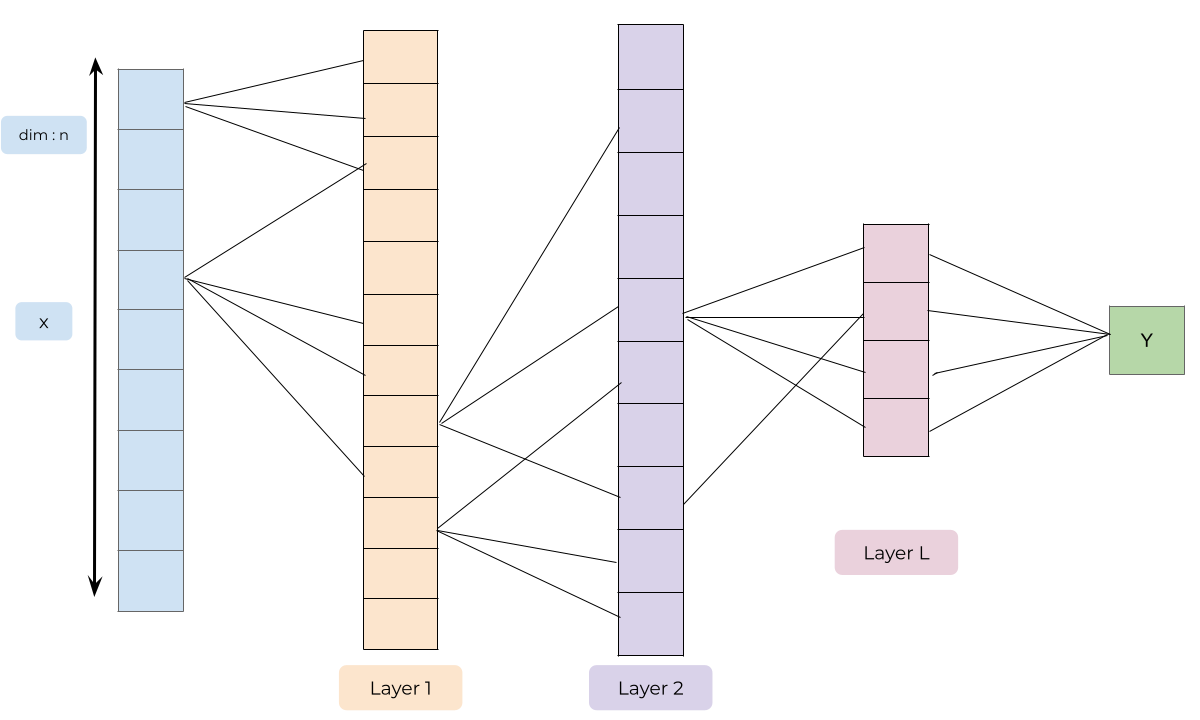
\includegraphics[width=0.9\linewidth]{images/NeuralNetwork} 
}
\end{figure}
\end{frame}

%#######################################


\begin{frame}{About \(d\) and \(e\) : neural networks}
\protect\hypertarget{about-d-and-e-neural-networks}{}
\begin{figure}

{\centering 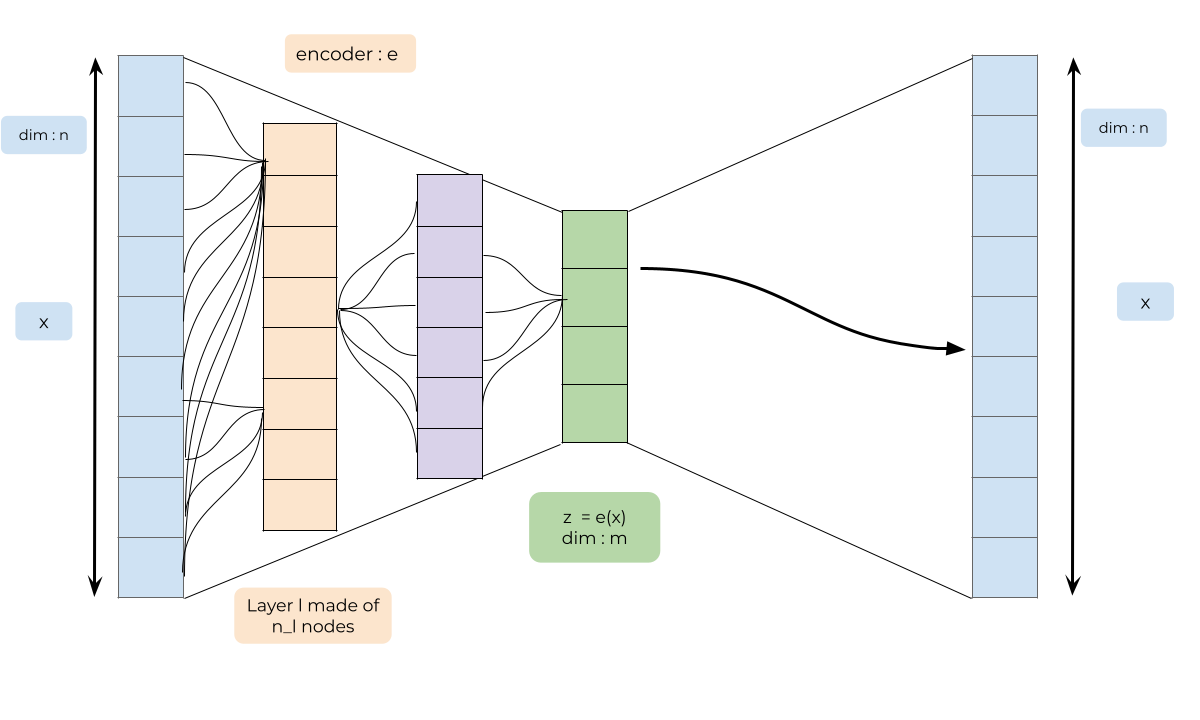
\includegraphics[width=0.9\linewidth]{images/Autoencoder2} 

}
\end{figure}
\end{frame}

%#######################################



\begin{frame}{About neural networks}
\protect\hypertarget{about-neural-networks}{}
\textbf{One neuron} :
\(f_j (\mathbf{X}) = \phi (<w_j, \mathbf {x}> + \, b_j)\) where

\begin{itemize}
\item
  \(\phi\) the activation function : non linear
\item \(w_j = (w_j^1, \dots, w_j^n)\) are the weights of the
  input variables \((x^1, \dots, x^n)\)
\item
  \(b_j\) is the bias of neuron \(j\).
\end{itemize}

\textbf{At each layer} \(\ell\) of the neural network:

\begin{itemize}
\item
  Receive \(n_{\ell-1}\) input variables
  \(\mathbf{y}^{\ell-1} =(y^{\ell-1}_{1}, \dots,y^{\ell-1}_{n_{\ell-1}})\)
\item
  Create \(n_\ell\) new variables. For variable \(j\) of layer \(l\):
  \[y^{\ell}_{j} = \phi(<w^\ell_j, \mathbf{y}^{\ell-1}>  +  b^{\ell}_j)\]
\end{itemize}

\textbf{Unknown parameters} \(\theta\)
\begin{itemize}
\item  \(w^\ell_j \in \mathbb{R}^{n_\ell-1}\), for \(\ell =1, \dots L\), for
\(j=1,\dots,n_{\ell}\), 
\item \(b^\ell_j \in \mathbb{R}\), for
\(\ell =1, \dots L\), for \(j=1,\dots,n_{\ell}\),
\end{itemize}
\end{frame}


%#######################################

\begin{frame}{Model choice}
\protect\hypertarget{model-choice}{}
\textbf{To choose}:

\begin{itemize}
\item
  The number of layers \(L\)
\item
  The number of neurons in each layer: \(n_\ell\) :
\item
  possibly \(n_\ell > n\)
\item
  For \textbf{autoencoder} the middle layer \(m < n\)
\item
  The activation function \(\phi\) (possibly one for the hidden layers $\phi$ and one $\psi$ for the activation layer)
\end{itemize}
\end{frame}
%#######################################


\begin{frame}{Learning \(f,d\) and \(e\)}

\begin{itemize}
\item
  \textbf{Regression or classification}
\end{itemize}

\(\theta = (w^\ell_j,b^\ell_j)_{j = 1\dots,n_\ell, \ell = 1,\dots,L}\)
are calibrated on a dataset \((X_i,Y_i)_{i=1, \dots , N_{obs}}\) by
minimizing the loss function

\[\widehat{\theta} = \mbox{argmin}_{\theta \in\Theta}  \sum_{i=1}^{N_{obs}}\mbox{Loss}(Y_i - f_{\theta}(X_i))\]

\begin{itemize}

\item  \textbf{Autoencoder}
\end{itemize}

\(\theta = (w^\ell_j,b^\ell_j)_{j = 1\dots,n_\ell, \ell = 1,\dots,L}\)
are calibrated on a dataset \((X_i)_{i=1, \dots , N_{obs}}\) by
minimizing the loss function

\[\widehat{\theta} = \mbox{argmin}_{\theta \in\Theta}  \sum_{i=1}^{N_{obs}}||X_i - d_{\theta}\circ e_{\theta}(X_i)||^2\]

\textbf{Optimisation by Stochastic gradient descent}: see later for a
reminder of the principle
\end{frame}

%#######################################

\subsection{PCA versus autoencoder}
\begin{frame}{PCA versus autoencoder}
\protect\hypertarget{pca-versus-autoencoder}{}
\begin{itemize}
\item
  Let \(P \in M_{n,m}(\mathbb{R})\),%\(W = (C_1,\dots,C_m)\)
%\item
 % The \(C_i\)'s are \(m\) columns vectors, \(m < n\).
\item
  \textbf{Hyp.}: %\((C_i)\) are orthonormal vectors. Consequently:
  \[P'P = I_n\]
\item
  Let \(P' X_i\) is the projector of vector \(X_i\) on the sub-vectorial
  space generated by the columns of \(P\).
\item
  We are looking for \(P\) minimizing the inertia of the projected
  dataset: \[
  \begin{aligned}
  \widehat{P} &=\mbox{argmax}_{\{P\in M_{n,m}(\mathbb{R}), P'P = I_n\}} \sum_{i=1}^{N_{obs}} || P'X_i||^2\\ &=\mbox{argmin}_{\{P \in M_{n,m}(\mathbb{R}), P'P = I_n\}} \sum_{i=1}^{N_{obs}} || X_i - PP'X_i||^2
  \end{aligned}
  \]
\end{itemize}
\end{frame}


%##################################################''

\begin{frame}{PCA versus autoencoder}
\protect\hypertarget{pca-versus-autoencoder-1}{}
\begin{itemize}
\item
  \(W' = e\) : \textbf{linear} encoder function
\item
  \(W = d\) : \textbf{linear} decoder function
\item
  Note that if you use neural networks with linear activation function
  and one layer, you will get \(W\) not necessarily orthogonal.
\end{itemize}

\href{http://www.xavierdupre.fr/app/mlstatpy/helpsphinx/c_ml/rn/rn_9_auto.html}{Lien
vers une démonstration propre}
\end{frame}


%#######################################
\subsection{A few reminder on the optimization procedure}
%#######################################

\begin{frame}{Minimization by Stochastic gradient descent.}

\textbf{Algorithm (by Rumelhart et al (1988))}

\begin{itemize}
\item
  Choose an initial value of parameters \(\theta\) and a learning rate
  \(\rho\)
\item
  Repeat until a minimum is reached:

  \begin{itemize}
  
  \item
    Split randomy the training set into \(N_B\) \emph{batches} of size
    \(b\) (\(n = b \times N_B\))
  \item
    for each batch \(B\) set:
    \[ \theta:= \theta - \rho \frac{1}{b}\sum_{i \in B} \nabla_{\theta} \left\{  \text{Loss}(f(\mathbf{X}_i,\theta),Y_i) \right\}\]
  \end{itemize}
\end{itemize}

\textbf{Remarks}:

\begin{itemize}
\item
  Each iteration is called an \emph{epoch}.
\item
  The number of epochs  and batches are  parameters  to tune
\item
  Difficulty comes from the computation of the gradient
\end{itemize}

\end{frame}
%#######################################
\begin{frame}{Calculus of the gradient for the regression}
\protect\hypertarget{calculus-of-the-gradient-for-the-regression}{}

\begin{itemize}

\item
  \(Y \in \mathbb{R}\).
\item
  \(R_i = \text{Loss}(f(\mathbf{X}_i,\theta),Y_i) = (Y_{i} - f(\mathbf{X}_i,\theta))^2\)
\item
  For any activation function \(\phi\) (hidden layers) and \(\psi\)
\end{itemize}

\end{frame}
%#######################################
\begin{frame}{Partial derivatives of \(R_i\) with respect to the weights
of the last layer}


\begin{itemize}
\item
  Derivatives of
  \(R_i = \left(Y_{i} - f(\mathbf{X}_i,\theta)\right)^2= \left(Y_i - h^{(L+1)}(\mathbf{X}_i)\right)^2\)
  with respect to \((w_j^{(L+1)})_{j=1\dots J_{L}}\)
\item
  \(a^{(L+1)}(\mathbf{X}) = b^{(L+1)} +w^{(L+1)} h^{(L)}(\mathbf{X}) \in \mathbb{R}^J\)
\item
  \begin{eqnarray*}
  f(\mathbf{X} ,\theta) &=& h^{(L+1)}(\mathbf{X}) \\
  &=& \psi(a^{(L+1)}(\mathbf{X}))  \\
  & =& \psi\left(b^{(L+1)} +\sum_{j=1}^{J_L} w_j^{(L+1)} h_j^{(L)}(\mathbf{X}) \right)
  \end{eqnarray*}
\item
  \[ \frac{\partial R_i }{\partial w^{(L+1)}_{j}} = -2\left(Y_{i} - f(\mathbf{X}_i,\theta)\right)\psi'\left(a^{(L+1)}(\mathbf{X}_i)\right)h_j^{(L)}(\mathbf{X}_i)\]
\end{itemize}

\end{frame}
%#######################################
\begin{frame}{Partial derivatives of \(R_i\) with respect to the weights
of the layer \(L-1\)}
\protect\hypertarget{partial-derivatives-of-r_i-with-respect-to-the-weights-of-the-layer-l-1}{}

\begin{itemize}
\item
  Derivatives of \(R_i = \left(Y_i - h^{(L+1)}(\mathbf{X}_i)\right)^2\)
  with respect to \((w_{jm}^{(L)})_{j=1\dots J_{L},m=1\dots J_{L-1}}\)
\item
  \begin{eqnarray*}
  \frac{\partial R_i }{\partial w^{(L)}_{jm}} &=& -2\left(Y_{i} - f(\mathbf{X}_i,\theta)\right)\psi'\left(a^{(L+1)}(\mathbf{X}_i)\right) \frac{\partial}{\partial w^{(L)}_{jm}}  a^{(L+1)}(\mathbf{X}_i)
  \end{eqnarray*}
\end{itemize}

\end{frame}
%#######################################
\begin{frame}{Partial derivatives of \(R_i\) with respect to the weights
of the layer \(L-2\)}
\protect\hypertarget{partial-derivatives-of-r_i-with-respect-to-the-weights-of-the-layer-l-2}{}

\begin{eqnarray*}
a^{(L+1)}(\mathbf{X}) &=&  b^{(L+1)} + \sum_{j=1}^{J_L} w^{(L+1)}_j h_j^{(L)}(\mathbf{X}) \\
&=&  b^{(L+1)} + \sum_{j=1}^{J_L}  w^{(L+1)}_j \phi \left(b_j^{(L)} + \sum_{m=1}^{J_{L-1}} w^{(L)}_{jm} h_m^{(L-1)}(\mathbf{X})\right)
\end{eqnarray*}

\begin{eqnarray*}
\frac{\partial}{\partial w^{(L)}_{jm}}  a^{(L+1)}(\mathbf{X}_i)  &=&   w^{(L+1)}_j \phi' \left(b_j^{(L)} + \sum_{m=1}^{J_{L-1}} w^{(L)}_{jm} h_m^{(L-1)}(\mathbf{X}_i)\right) \\
&& \times h_m^{(L-1)}(\mathbf{X}_i)   \\
&=& w^{(L+1)}_j \phi'(a_j^{L}(\mathbf{X}_i)) h_m^{(L-1)}(\mathbf{X}_i)
\end{eqnarray*}

\end{frame}
%#######################################
\begin{frame}{Forward-Backward algorithm (at each iteration)}
\protect\hypertarget{forward-backward-algorithm-at-each-iteration}{}

After some light effort, recurrence formula

\begin{itemize}

\item
  Given the current parameters

  \begin{itemize}
  
  \item
    \textbf{Forward step} : From layer \(1\) to layer \(L+1\), compute
    the \(a_j^{\ell}(\mathbf{X}_i),\phi(a_j^{\ell}(\mathbf{X}_i))\)\\
  \item
    \textbf{Backward step } : From layer \(L+1\) to layer \(1\), compute
    the partial derivatives (recurrence formula update)
  \end{itemize}
\end{itemize}

\end{frame}
%#######################################
\begin{frame}{Tuning the algorithm}
 

\begin{itemize}
 
\item
  \(\rho\): learning rate of the gradient descent

  \begin{itemize}
  
  \item
    if \(\rho\) too small, really slow convergence with possibly
    reaching of a local minimum\\
  \item
    if \(\rho\) too large, maybe oscilliation around an optimum without
    stabilisation
  \item
    Adaptive choice of \(\rho\) (decreasing $\rho$)
  \end{itemize}
\item
  Batch calculation reduces the number of quantities to be stored in the
  forward / backward
\end{itemize}

\end{frame}
%#################################################``
\begin{frame}{Obviously}
\protect\hypertarget{obviously}{}

Many improved versions of the maximisation algorithm (momentum
correction, Nesterov accelerated gradient, etc\ldots{})

\end{frame}

\begin{frame}[fragile]{Automatic differentiation}
\protect\hypertarget{automatic-differentiation}{}

Success of the neural network comes from automatic differentiation,
i.e.~automatisation of the previously described forward-backward
procedure to compute the derivatives : \texttt{Tensorflow}

\end{frame}


%#######################################
\section{Variational versions of neural networks}

\subsection{Motivations}

\begin{frame}{Why variational neural networks?}

  \textbf{Regression-Classification} : Bayesian inference of the
  parameters \(\theta\)
\begin{itemize}
\item
   Prior on \(\theta\): \(\pi(\theta)\)
\item
  Estimation not of \(\theta\) but of the posterior distribution of
  \(\theta\) : \(p(\theta | \mathbf{Y})\)
\end{itemize}

  \textbf{Autoencoder}: give a structure on the latent space
  \(\mathbf{Z}\)
  
\begin{itemize}

\item
  Distribution  on \(Z\): \(\pi(Z)\)
\item
  \textbf{Point estimation} of \(\theta\) and \textbf{estimation of  the posterior distribution of \(Z\) :
  \(p(Z | \theta, \mathbf{X})\)}
\end{itemize}


 \textbf{Variational} : approximation of the distributions
\begin{itemize}
 \item
  \(p(\theta | \mathbf{Y}) \approx q_\mathbf{Y}(\theta)\)
\item
  \(p(Z | \theta, \mathbf{X}) \approx q_\mathbf{X}(Z)\)
\end{itemize}
\end{frame}


\begin{frame}{Using the autoencoder to simulate}
\protect\hypertarget{using-the-autoencoder-to-simulate}{}
\begin{center}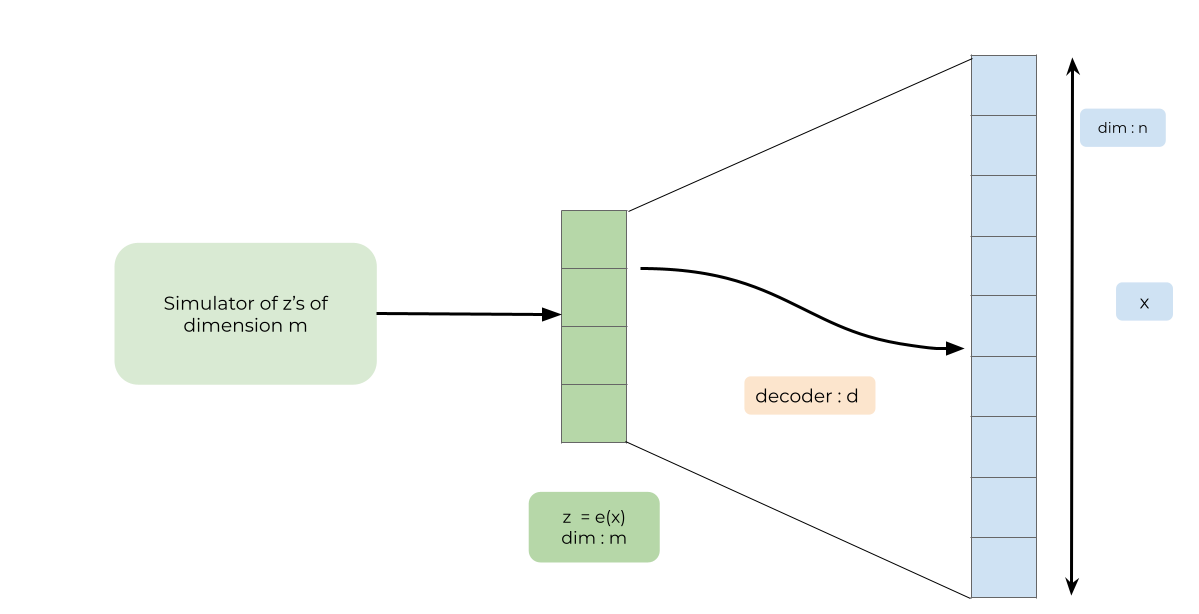
\includegraphics[width=0.7\linewidth]{images/VarAutoencoder} \end{center}

\begin{itemize}
\item
  The optimization of the autoencoder supplies
  \((Z_1, \dots, Z_{N_{obs}}) = (e(x_1), \dots, e(X_{N_{obs}}))\)
\item
  \textbf{How can we simulate the} \(z's\) such that \(d(z)\) looks like
  my original data?
\item
  How to construct a ``machine'' able to generate coherent other
  \(Z_i\).
\item
  Need to constrain/ structure the latent space.
\end{itemize}
\end{frame}


%#######################################

\begin{frame}{Probabilistic version of the autoencoder}
\protect\hypertarget{probabilistic-version-of-the-autoencoder}{}
\begin{itemize}
\item
  \textbf{Idea} : put a probabilistic distribution on the latent space and
  estimate the posterior distribution.
\item
  \textbf{A statistical model with latent variables}
\end{itemize}

\[X_i =d(Z_i) + \epsilon_i\] \[Z_i \sim_{i.i.d.}N_m(0,I_m)\]
\[\epsilon_i \sim_{i.i.d.} \mathcal{N}_n(0,c I_n)\]

\begin{itemize}
\item
  Likelihood
  \[\ell(\mathbf{X}; d)  =  \int_{\mathbf{Z}} p(\mathbf{X} | \mathbf{Z};d)p(\mathbf{Z})d\mathbf{Z}\]
\end{itemize}

\textbf{Not explicit}

\begin{itemize}
\item
  EM requires the posterior distribution of \(\mathbf{Z}\)
\end{itemize}

\[p(\mathbf{Z} | \mathbf{X}; d) \propto p(\mathbf{X}|\mathbf{Z}; d)p(\mathbf{Z}) \]
\textbf{Very complex too}
\end{frame}

%#######################################


\subsection{Variational bayesian inference}

\begin{frame}{Principal of variational Bayesian inference}
\protect\hypertarget{variational-bayesian-inference}{}
\begin{itemize}
\item
  Approximate the posterior \(p(\theta | Y)\) by \(q(\theta)\) where
  \(q\in \mathcal{R}\)
\item
  \(\mathcal{R}\) family of simpler distributions. \textbf{Example}:
  \(q(\cdot) = \mathcal{N}(\mu,\Sigma)\)
\item
  Approximating = Minimizing
  \[ D_\text{KL}(q(\theta),p(\theta | \mathbf{Y})) = \mathbf{E}_q\left[\log \frac{q(\theta)}{p(\theta | \mathbf{Y})}\right]\]
\end{itemize}
\end{frame}
 %#################################################``
\begin{frame}{The Magik trick}



$$D_\text{KL}(q(\theta),p(\theta | \mathbf{Y}))  = \log \ell(\mathbf{Y}) + \left[ - \underbrace{\mathbf{E}_q[\log \ell(\mathbf{Y}|\theta)\pi(\theta)] +\mathbf{E}_q[\log q(\theta)]}_{\mathcal{F}(q)}\right]$$ 

\begin{itemize}
 \item \(\log \ell(\mathbf{Y})\) independent of \(q\)
\item   Minimizing the Kullback–Leibler divergence  w.r. to $q$ is
equivalent to minimizing $\mathcal{F}(q)$ with respect to $q$

\end{itemize}


\begin{eqnarray}
\mathcal{F}(q) &=& -  \mathbf{E}_q[\log \ell(\mathbf{Y}|\theta)\pi(\theta)] + \mathbf{E}_q[\log q(\theta)] \\
&=&  -  \mathbf{E}_q[\log \ell(\mathbf{Y}|\theta)] + \mathbf{E}_q\left[\log \frac{q(\theta)}{\pi(\theta)}\right] \\
&=&D_{\text{KL}}(q,\pi) -  \mathbf{E}_q[\log \ell(\mathbf{Y}|\theta)]   
\end{eqnarray}

\end{frame}

 %#################################################``
\begin{frame}{Parametrization of $q$}



Choose a \textbf{parametric} form in $q = q_{\eta}$. 
  
  \begin{itemize}
 \item For example: $q = \mathcal{N}(\mu,\Sigma)$ 
\end{itemize}

$$\hat{\eta} = \arg\min_{\eta} \mathcal{F}(\eta) = \arg\min_{\eta} D_{\text{KL}}(q_{\eta},\pi) - \mathbf{E}_{q_{\eta}}[\log \ell(\mathbf{Y}|\theta)]$$

\begin{itemize}
 \item Optimisation by gradient descent
  \item   \textbf{BUT} expectation not explicit
  \end{itemize}
\end{frame}

%#################################################``
\begin{frame}{Monte Carlo approximation}
 

\begin{itemize}
 \item With neural networks, $\mathbf{E}_{q_{\eta}}[\log \ell(\mathbf{Y}|\theta)]$  not explicit (activation functions non linear)
  
 \item Approximation by Monte Carlo :  assume that $\theta^{(m)} \sim q_{\eta}$, $m = 1,\dots, M$
  
$$\widehat{\mathcal{F}}(\eta) = \frac{1}{M}\sum_{m=1}^M  \log \frac{q_{\eta}(\theta ^{(m)})}{\pi(\theta^{(m)})} -  \log \ell(\mathbf{Y}|\theta^{(m)})$$
  
  \item \textbf{Problem}:  we lost the explicit dependence in $\eta$ through the simulations  $\theta^{(m)}$ 
  
  \item \textbf{Solution} : reparametrisation $$\xi^{(m)}\sim \mathcal{N}(0,\mathbf{I})  \quad \mbox{and} \quad \theta^{(m)} = \phi(\xi^{(m)},{\color{orange}\eta} )$$
$$\widehat{\mathcal{F}}(\eta) = \frac{1}{M}\sum_{m=1}^M   \log q_{\eta}(\phi(\xi^{(m)},\eta)) - \log \pi(\phi(\xi^{(m)},\eta)) - \log \ell(\mathbf{Y}| \phi(\xi^{(m)},\eta))$$
\end{itemize}
\end{frame}

%#################################################``
\begin{frame}{Remarks}
$$\widehat{\mathcal{F}}(\eta) = \frac{1}{M}\sum_{m=1}^M   \log q_{\eta}(\phi(\xi^{(m)},\eta)) - \log \pi(\phi(\xi^{(m)},\eta)) - \log \ell(\mathbf{Y}| \phi(\xi^{(m)},\eta))$$

 \begin{itemize}
 \item  People take $M=1$  
  \item  $D_{\text{KL}}(q_{\eta},\pi)$ may be explicit (for Gaussian distributions for instance) but not used in practice
  \item  $\xi^{(m)}$ are resimulated each time we compute the gradients
  \end{itemize}
\end{frame}
  
%#################################################``
\begin{frame}{More details for the regression case}

\begin{itemize}
 \item $\theta$ are the parameters (weights and bias)
 \item Prior gaussian distribution on $\theta$ : $\theta \sim \mathcal{N}(0, \mathbb{I})$
 \item If regression  $Y_i = f_\theta(X_i) + \epsilon_i, \quad \epsilon \sim \mathcal{N}(0,\sigma^2)$ 
 $$-\ell(\bY,\phi(\xi^{(m)},\eta)) = \left[\sum_{i=1}^{N_{obs}}   \frac{||Y_i - f_{ \phi(\xi^{(m)},\eta) }(X_i)||^2}{2\sigma^2}\right]$$ 
 
\end{itemize}



\end{frame}

\subsection{Variational (probabilistic)
autoencoder}
%#######################################


\begin{frame}{The problem}

\begin{eqnarray*}
 \mathbf{X}_i &=&d_\theta(Z_i) + \epsilon_i \\
 Z_i &\sim&_{i.i.d.}N_m(0,I_m)\\
 \epsilon_i &\sim&_{i.i.d.} \mathcal{N}_n(0,\sigma^2 I_n)
\end{eqnarray*}

Likelihood
  \[\ell(\mathbf{X}; d_{\theta})  =  \int_{\mathbf{Z}} \ell(\mathbf{X} | \mathbf{Z};d_\theta)p(\mathbf{Z})d\mathbf{Z}\]

No explicit form, linked ot the fact that $p(\mathbf{Z}  | \mathbf{X};d_{\theta})$ is complex
  
\end{frame}

\begin{frame}{The Evidence Lower BOund (ELBO)}

\begin{itemize}

\item

Let's simplify that distribution 
$p(\mathbf{Z}  | \mathbf{X};d_{\theta})$ 
\begin{eqnarray*}
 p(\mathbf{Z}  | \mathbf{X};d_{\theta}) &=& q_{\mathbf{X}}(\mathbf{Z};g,H)\\
 \prod_{i=1}^{N_{obs}} p(Z_i |  X_i; d_{\theta}) &\approx&     \prod_{i=1}^{N_{obs}} q_{ X_i}(Z_i;g,H)\\
 q_{X_i}(Z_i;g,h) &=&\mathcal{N}_m(g(\textbf{X}_i),H(g(\textbf{X}_i))
 \end{eqnarray*}
 
 where $g$ and $H$ are chosen such that 
$D_\text{KL}(q(\mathbf{Z};\mathbf{X},g,H), p(\mathbf{Z} |\mathbf{X};d_\theta))$ is small

\item
  Replace the likelihood by the ELBO


\begin{eqnarray*}
\text{ELBO}(d_{\theta},g,H) &=&\ell(\mathbf{X}; d_{\theta})-  D_\text{KL}(q(\mathbf{Z};\mathbf{X},g,H), p(\mathbf{Z} |\mathbf{X};d))\\
%&=&\mathbb{E}_{q_{\mathbf{X}}(\mathbf{Z}; ,g,H)}[\log p(\mathbf{X} , \mathbf{Z};d)] + Entr(q_{\mathbf{X}}(\mathbf{Z};g,H)))\\
&=& \mathbb{E}_{q_{\mathbf{X}}(\mathbf{Z};g,H)}[\log p(\mathbf{X} | \mathbf{Z};d_{\theta})]- D_\text{KL}(q_{\mathbf{X}}(\mathbf{Z};g,H), p(\mathbf{Z}))
\end{eqnarray*}

\end{itemize}

\end{frame}
%"#########################################################
\begin{frame}{Optimization: minimize $-\text{ELBO}(d,g,H) $ }
 


\[-\text{ELBO}(d,g,H)  =-  \mathbb{E}_{q_{\mathbf{X}}(\mathbf{Z};g,H)}[\log p(\mathbf{X} | \mathbf{Z};d_\theta)] +  D_\text{KL}(q_{\mathbf{X}}(\mathbf{Z};g,h), p(\mathbf{Z}))\]

\begin{itemize}
\item \textbf{Reconstruction} term 

$$-\mathbb{E}_{q_{\mathbf{X}}(\mathbf{Z};g,H)}[\log p(\mathbf{X} | \mathbf{Z};d_\theta)] = \mathbb{E}_{q_{\mathbf{X}}(\mathbf{Z};g,H)}  \left[\sum_{i=1}^{N_{obs}}   \frac{||\mathbf{X}_i - d_\theta(Z_i)||^2}{2\sigma^2}\right]$$ 

\item \textbf{Regularisation} term :  $D_\text{KL}$
  
\item  $\sigma^2$ : variance parameter which balances regularisation and  reconstruction
\end{itemize}
\end{frame}
%"#########################################################

\begin{frame}[fragile]{About $d_\theta$, $g$ and $H$}
  
$d_\theta$ neural network function as before   

About $g$ and $H$ : called the "encoder part"
 
\begin{itemize}
\item    $H(X)$ is a covariance so
\begin{itemize}
\item  it should be a square symmetric matrix
\item  \textbf{Simplification}: diagonal matrix $H(\mathbf{X}) = diag(h^2(X))$ where  $h(X) \in \mathbb{R}^m$
\end{itemize}
\item
  \(h(\mathbf{X}) = h_2(h_1(\mathbf{X}))\), \(g(\mathbf{X}) = g_2(g_1(\mathbf{X}))\), \(g_1 = h_1\)
  \item $g_2$,$g_2$, $h_1$ neural networks 
\end{itemize}

\begin{center}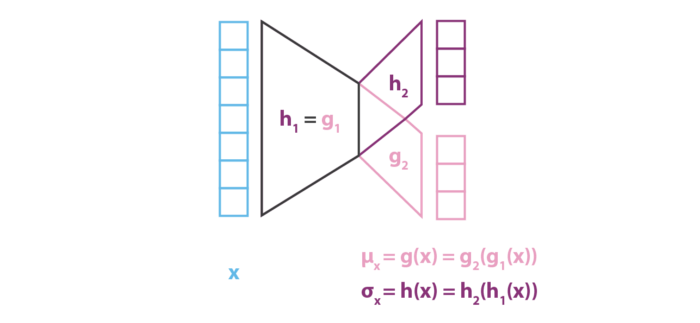
\includegraphics[width=0.7\linewidth]{images/approxZ} \end{center}

\end{frame}
%#########################################################


\begin{frame}{About the expectation}
\begin{itemize}
 \item \(\mathbb{E}_{q_{\mathbf{X}}(\mathbf{Z};g,h)} \left[\sum_{i=1}^{N_{obs}}  \frac{||\mathbf{X}_i - d_{\theta}(Z_i)||^2}{2\sigma^2}\right]\)
can not be evaluated.


\item Monte Carlo approximation on $1$ realization
\item Reparametrisation trick 

$$Z_i^{sim} = g(X_i) + diag(h(X_i))\zeta_i, \quad \mbox{ with } \xi_i\sim \mathcal{N}_m(0,\mathbb{I}_m)$$
\end{itemize}


\begin{eqnarray*}
 \mathbb{E}_{q_{\mathbf{X}}(\mathbf{Z};g,h)}  \left[\sum_{i=1}^{N_{obs}}   \frac{||\mathbf{X}_i - d_{\theta}(Z_i)||^2}{2\sigma^2}\right] \approx  \sum_{i=1}^{N_{obs}} \frac{||\mathbf{X}_i - d_{\theta}(Z^{(sim)}_i)||^2}{2\sigma^2}\\
  \sum_{i=1}^{N_{obs}} \frac{||\mathbf{X}_i - d_{\theta}(g(X_i) + diag(h(X_i))\zeta_i)||^2}{2\sigma^2}
\end{eqnarray*}



\end{frame}
\begin{frame}{Finally...}
\begin{center}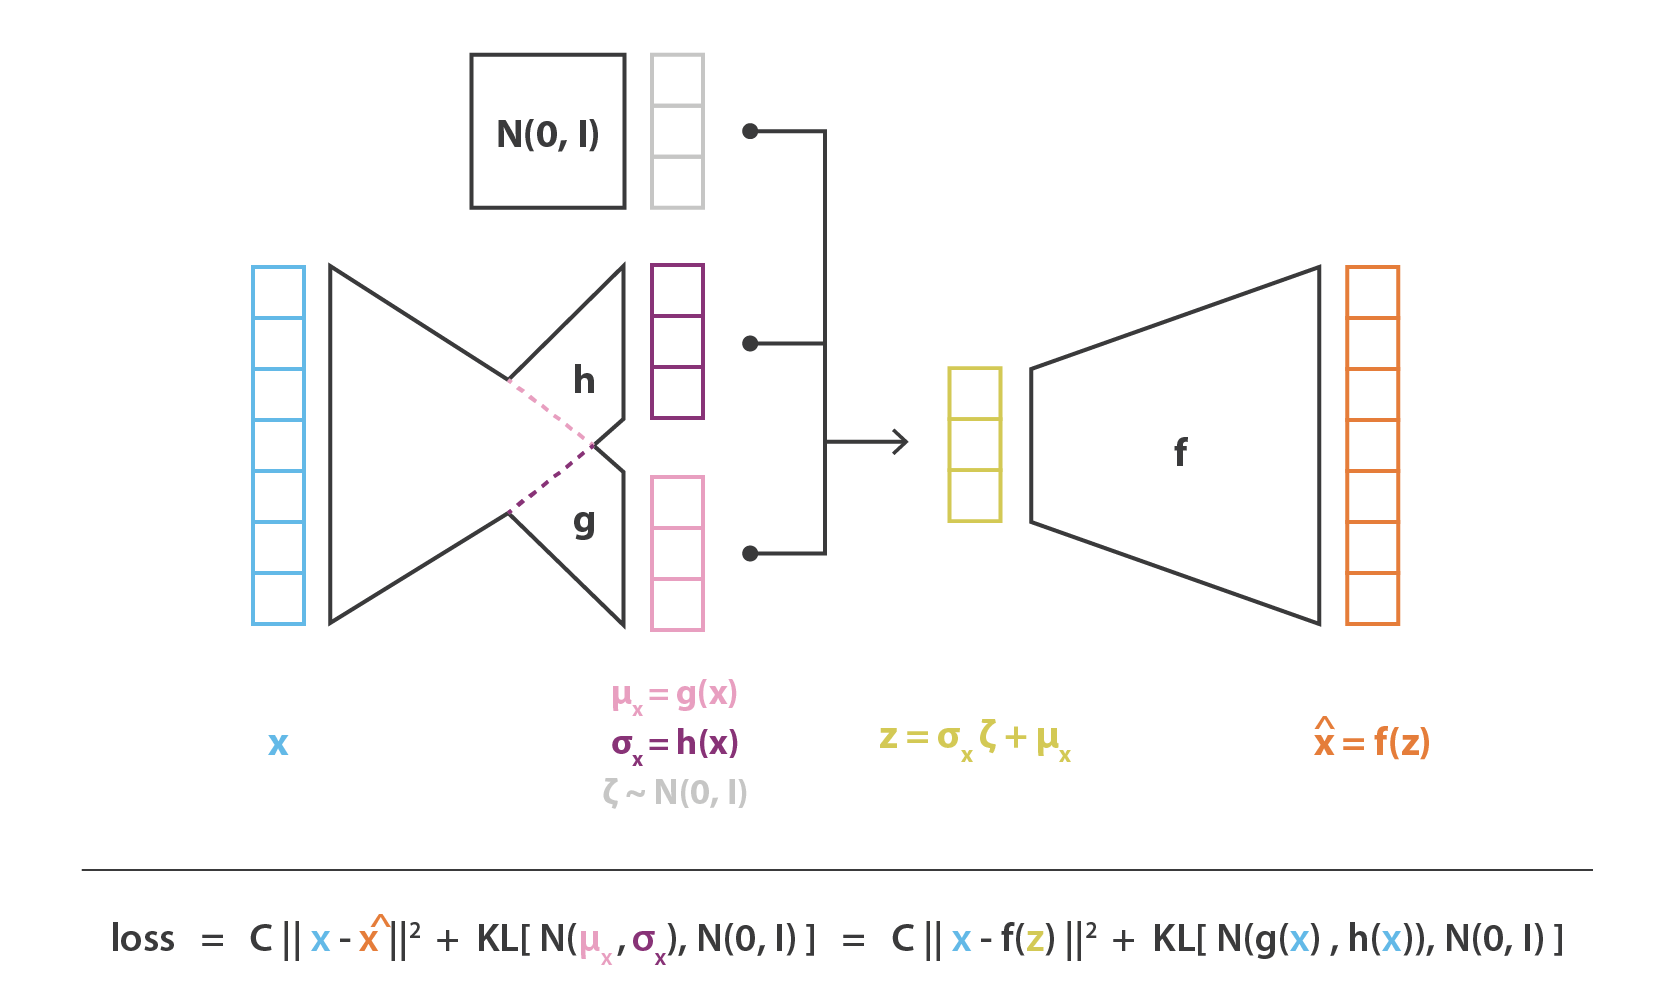
\includegraphics[width=0.8\linewidth]{images/varAutoencoderAll} \end{center}
 
\end{frame}

%#########################################################


\begin{frame}{Conclusion}

\begin{itemize}
 \item Easy to understand all the tools
 \item Now, how easy is it to encode this? 
\end{itemize}


\end{frame}
\end{document}
